\documentclass[aspectratio=169]{beamer}

%\setbeameroption{hide notes}
%\setbeameroption{show notes}
%\setbeameroption{show only notes}

% Copyright (C) 2012 - EDF R&D - Michael Baudin

% To highlight source code
\usepackage{listings}
\definecolor{darkgreen}{rgb}{0,0.5,0}
\definecolor{violet}{rgb}{0.5,0,1}

\usepackage{lmodern}% http://ctan.org/pkg/lm

\usetheme{Montpellier}
\setbeamertemplate{navigation symbols}{} % Remove navigation
\useoutertheme{infolines}

\usepackage[utf8]{inputenc}
\usepackage[T1]{fontenc}

%\usepackage[french]{babel}
%\uselanguage{French}
%\languagepath{French}

\def\bx{{\bf x}}
\def\RR{\mathbb{R}}

\newcommand{\pyvar}[1]{\texttt{#1}}

\def \ot {OpenTURNS}

\hypersetup{colorlinks=true}

\usepackage{adjustbox}

\date[]{UserDay \#15, 10 June 2022, EDF Lab Saclay}

%%%%%%%%%%%%%%%%%%%%%%%%%%%%%%%%%%%%%%%%%%%%%%%%%%%%%%%%%%%%%%%%%%%%%%%%%%%%%

\begin{document}

%%%%%%%%%%%%%%%%%%%%%%%%%%%%%%%%%%%%%%%%%%%%%%%%%%%%%%%%%%%%%%%%%%%%%%%%%%%%%

\begin{frame}
\frametitle{Variance-based sensitivity analysis for functional inputs}

\framesubtitle{Methodology}

We observe an application $h$ from $n$ fields $(\mat{X_1}, \dots, \mat{X_n})$ \\
of the associated input process $\mat{X}$ and $n$ vectors $(\vect{Y_1},\dots,\vect{Y_n})$

$$
h: \left|
  \begin{array}{ccl}
      \cM_N \times (\Rset^d)^N & \rightarrow & \Rset^p \\
      \mat{X} & \mapsto & \vect{Y}
  \end{array}
\right.
$$

\vspace{10mm}

We propose the following steps to lead to sensitivity analysis.

\begin{itemize}
\item 1. Identify blocks of independent inputs
\item 2. Dimension reduction via Karhunen-Loeve for each input block
\item 3. Approximate of the link between KL coefficients and vectorial outputs by chaos
\item 4. Post-process functional chaos coefficients to derive Sobol` indices
\end{itemize}

\end{frame}


\begin{frame}
\frametitle{Variance-based sensitivity analysis for functional inputs}

\framesubtitle{Methodology step 1/4: Identify blocks}

Identify groups of independent components in $\mat{X}$\\
by construction, if the underlying process is known


\end{frame}


\begin{frame}
\frametitle{Variance-based sensitivity analysis for functional inputs}

\framesubtitle{Methodology step 2/4: Dimension reduction by Karhunen-Loeve}

We use the Karhunen-Loeve decomposition to find the $(\lambda_k, \vect{\varphi}_k)_{k \geq 1}$ \\
solutions of the Fredhlom equation:

$$
\int_{\cD} \mat{C}(\vect{s},\vect{t}) \vect{\varphi}_k(\vect{t})\,  d\vect{t} = \lambda_k  \vect{\varphi}_k(\vect{s}) \quad \forall \vect{s} \in \cD
$$

The SVD decomposition helps to approach the covariance function $\mat{C}$ by its empirical estimator.

\end{frame}

\begin{frame}
\frametitle{Variance-based sensitivity analysis for functional inputs}

\framesubtitle{Methodology step 2/4: Dimension reduction by Karhunen-Loeve}

The linear projection function $\pi_{ \vect{\lambda}, \vect{\varphi}}$ of
the Karhunen-Loeve decomposition writes:

$$
    \pi_{\vect{\lambda}, \vect{\varphi}}: \left|
      \begin{array}{ccl}
        L^2(\cD, \Rset^d) & \rightarrow & \cS^{\Nset} \\
        f & \mapsto &\left(\dfrac{1}{\sqrt{\lambda_k}}\int_{\cD}f(\vect{t}) \vect{\varphi}_k(\vect{t})\, d\vect{t}\right)_{k \geq 1}
      \end{array}
    \right.
$$

This integral is replaced by a specific weighted and finite sum and to write the projections\\
of the j-th marginal of i-th input field $\vect{X_i^j}$ by multiplication\\
with the projection matrix $\mat{M^j} \in \Rset^{K_j} \times \Rset^{Nd}$:

$$
    \mat{M_j} \vect{X_i^j} = \left( \begin{array}{l} \xi_1^j \\ \dots \\ \xi_{K_j}^j \end{array} \right)
    \in \Rset^{K_j}, \forall i \in [1, n], \forall j \in [1, d]
$$

with $K_j$ the retained number of modes in the decomposition of the j-th input

\end{frame}

\begin{frame}
\frametitle{Variance-based sensitivity analysis for functional inputs}

\framesubtitle{Methodology step 2/4: Dimension reduction by Karhunen-Loeve}

The projections of all the $d$ components of $n$ fields are assembled in the $Q$ matrix:

$$
        \mat{Q} = \mat{M} \mat{X} =
        \left(
          \begin{array}{l}
            \mat{M_1} \mat{X^1} \\
            \dots \\
            \mat{M_d} \mat{X^d}
          \end{array}
        \right) \in \Rset^{K_T} \times \Rset^n
$$

with $K_T = \sum_{j=1}^d{K_j}$ the total number of modes accross input components

\end{frame}

\begin{frame}
\frametitle{Variance-based sensitivity analysis for functional inputs}

\framesubtitle{Methodology step 3/4: Link KL coefficients to ouputs}

Then a functional chaos decomposition is built between the projected modes\\
sample $\mat{Q}$ and the output samples $\mat{Y}$

$$
\tilde{g}(x) = \sum_{k=1}^{K_c} \beta_{\vect{\alpha}_k} \Psi_{\vect{\alpha}_k}(x)
$$

The final metamodel consists in the composition of the Karhunen-Loeve
projections and the functional chaos metamodel.

$$
    \tilde{h}: \left|
      \begin{array}{ccccl}
         \cM_N \times (\Rset^d)^N & \rightarrow & \Rset^{K_T} & \rightarrow & \Rset^p \\
         \mat{X} & \mapsto & \vect{Q} & \mapsto & \vect{Y}
      \end{array}
    \right.
$$

A limitation of this approach is that the projected modes sample has a dimension
$K_T$ so the dimension of the input fields $\mat{X_i}$
and the associated number of modes must remain modest.

\end{frame}


\begin{frame}
\frametitle{Variance-based sensitivity analysis for functional inputs}

\framesubtitle{Methodology step 3/4: Link KL coefficients to ouputs}

From the chaos decomposition:

$$
\tilde{g}(x) = \sum_{k=1}^{K_c} \beta_{\vect{\alpha}_k} \Psi_{\vect{\alpha}_k}(x)
$$

Lets expand the multi indices notation:

$$
    \Psi_{\vect{\alpha}}(x) = \prod_{j=1}^{K_T} P^j_{\alpha_j}(x_j)
$$

with $\alpha$ that contains the marginal degrees associated to the $K_T$ input components
$$
    \vect{\alpha} \in \mathbb{N}^{K_T} = \{\underbrace{\alpha_1, \dots, \alpha_{K_1}}_{K_1},\dots,\underbrace{\alpha_{K_T-K_d}, \dots, \alpha_{K_T}}_{K_d}\}
$$

\end{frame}


\begin{frame}
\frametitle{Variance-based sensitivity analysis for functional inputs}

\framesubtitle{Methodology step 4/4: Derive Sobol` indices from chaos coefficients}

Sobol indices of the input field component $j \in [1,d]$ can be computed
from the coefficients of the chaos decomposition that involve the
matching KL coefficients.

For the first order Sobol indices we sum over the multi-indices $\vect{\alpha}_k$
that are non-zero on the $K_j$ indices corresponding to the KL
decomposition of j-th input and zero on the other $K_T - K_j$ indices (noted $G_j$):

$$
S_j = \frac{\sum_{k=1, \vect{\alpha}_k \in G_j}^{K_c} \beta_{\vect{\alpha}_k}^2}{\sum_{k=1}^{K_c} \beta_{\vect{\alpha}_k}^2}
$$

For the total order Sobol indices we sum over the multi-indices $\vect{\alpha}_k$
that are non-zero on the $K_j$ indices corresponding to the KL
decomposition of the j-th input (noted $GT_j$):

$$
S_{T_j} = \frac{\sum_{k=1, \vect{\alpha}_k \in GT_j}^{K_c} \beta_{\vect{\alpha}_k}^2}{\sum_{k=1}^{K_c} \beta_{\vect{\alpha}_k}^2} 
$$

This generalizes to higher order indices.

\end{frame}


\begin{frame}[containsverbatim]
\frametitle{Variance-based sensitivity analysis for functional inputs}

\framesubtitle{API}

\lstset{language=python}
\begin{lstlisting}
algo = ot.FieldToPointFunctionalChaosAlgorithm(x, y)  # x~ProcessSample, y~Sample

# 1. KL parameters
algo.setCenteredSample(False)  # our input sample is not centered (default)
algo.setThreshold(4e-2)  # we expect to explain 96% of variance
algo.setRecompress(False)  # whether to re-truncate modes
algo.setNbModes(10) # max KL modes (default=unlimited)

# 2. chaos parameters:
ot.ResourceMap.SetAsUnsignedInteger('FunctionalChaosAlgorithm-BasisSize', N) # chaos basis size
algo.setSparse(True)

algo.setBlockIndices([[0], [1], [2, 3]])  # possibility to group inputs
algo.run()
\end{lstlisting}

\end{frame}


\begin{frame}[containsverbatim]
\frametitle{Variance-based sensitivity analysis for functional inputs}

\framesubtitle{API}

\lstset{language=python}
\begin{lstlisting}
result = algo.getResult()

# inspect eigen values
kl_results = result.getInputKLResultCollection()
n_modes = [len(res.getEigenvalues()) for res in kl_results]

# validate KL decompositions
for i in range(in_dim):
    View(ot.KarhunenLoeveValidation(x.getMarginal(i), kl_results[i]).drawValidation())

# inspect chaos residuals
print(result.getFCEResult().getResiduals())
print(result.getFCEResult().getRelativeErrors())

# validate chaos decomposition
validation = ot.MetaModelValidation(result.getModesSample(), result.getOutputSample(), result.getFCEResult().getMetaModel())
View(validation.drawValidation())

\end{lstlisting}

\end{frame}


\begin{frame}[containsverbatim]
\frametitle{Variance-based sensitivity analysis for functional inputs}

\framesubtitle{API}

\begin{figure}[!htb]
\minipage{0.5\textwidth}
  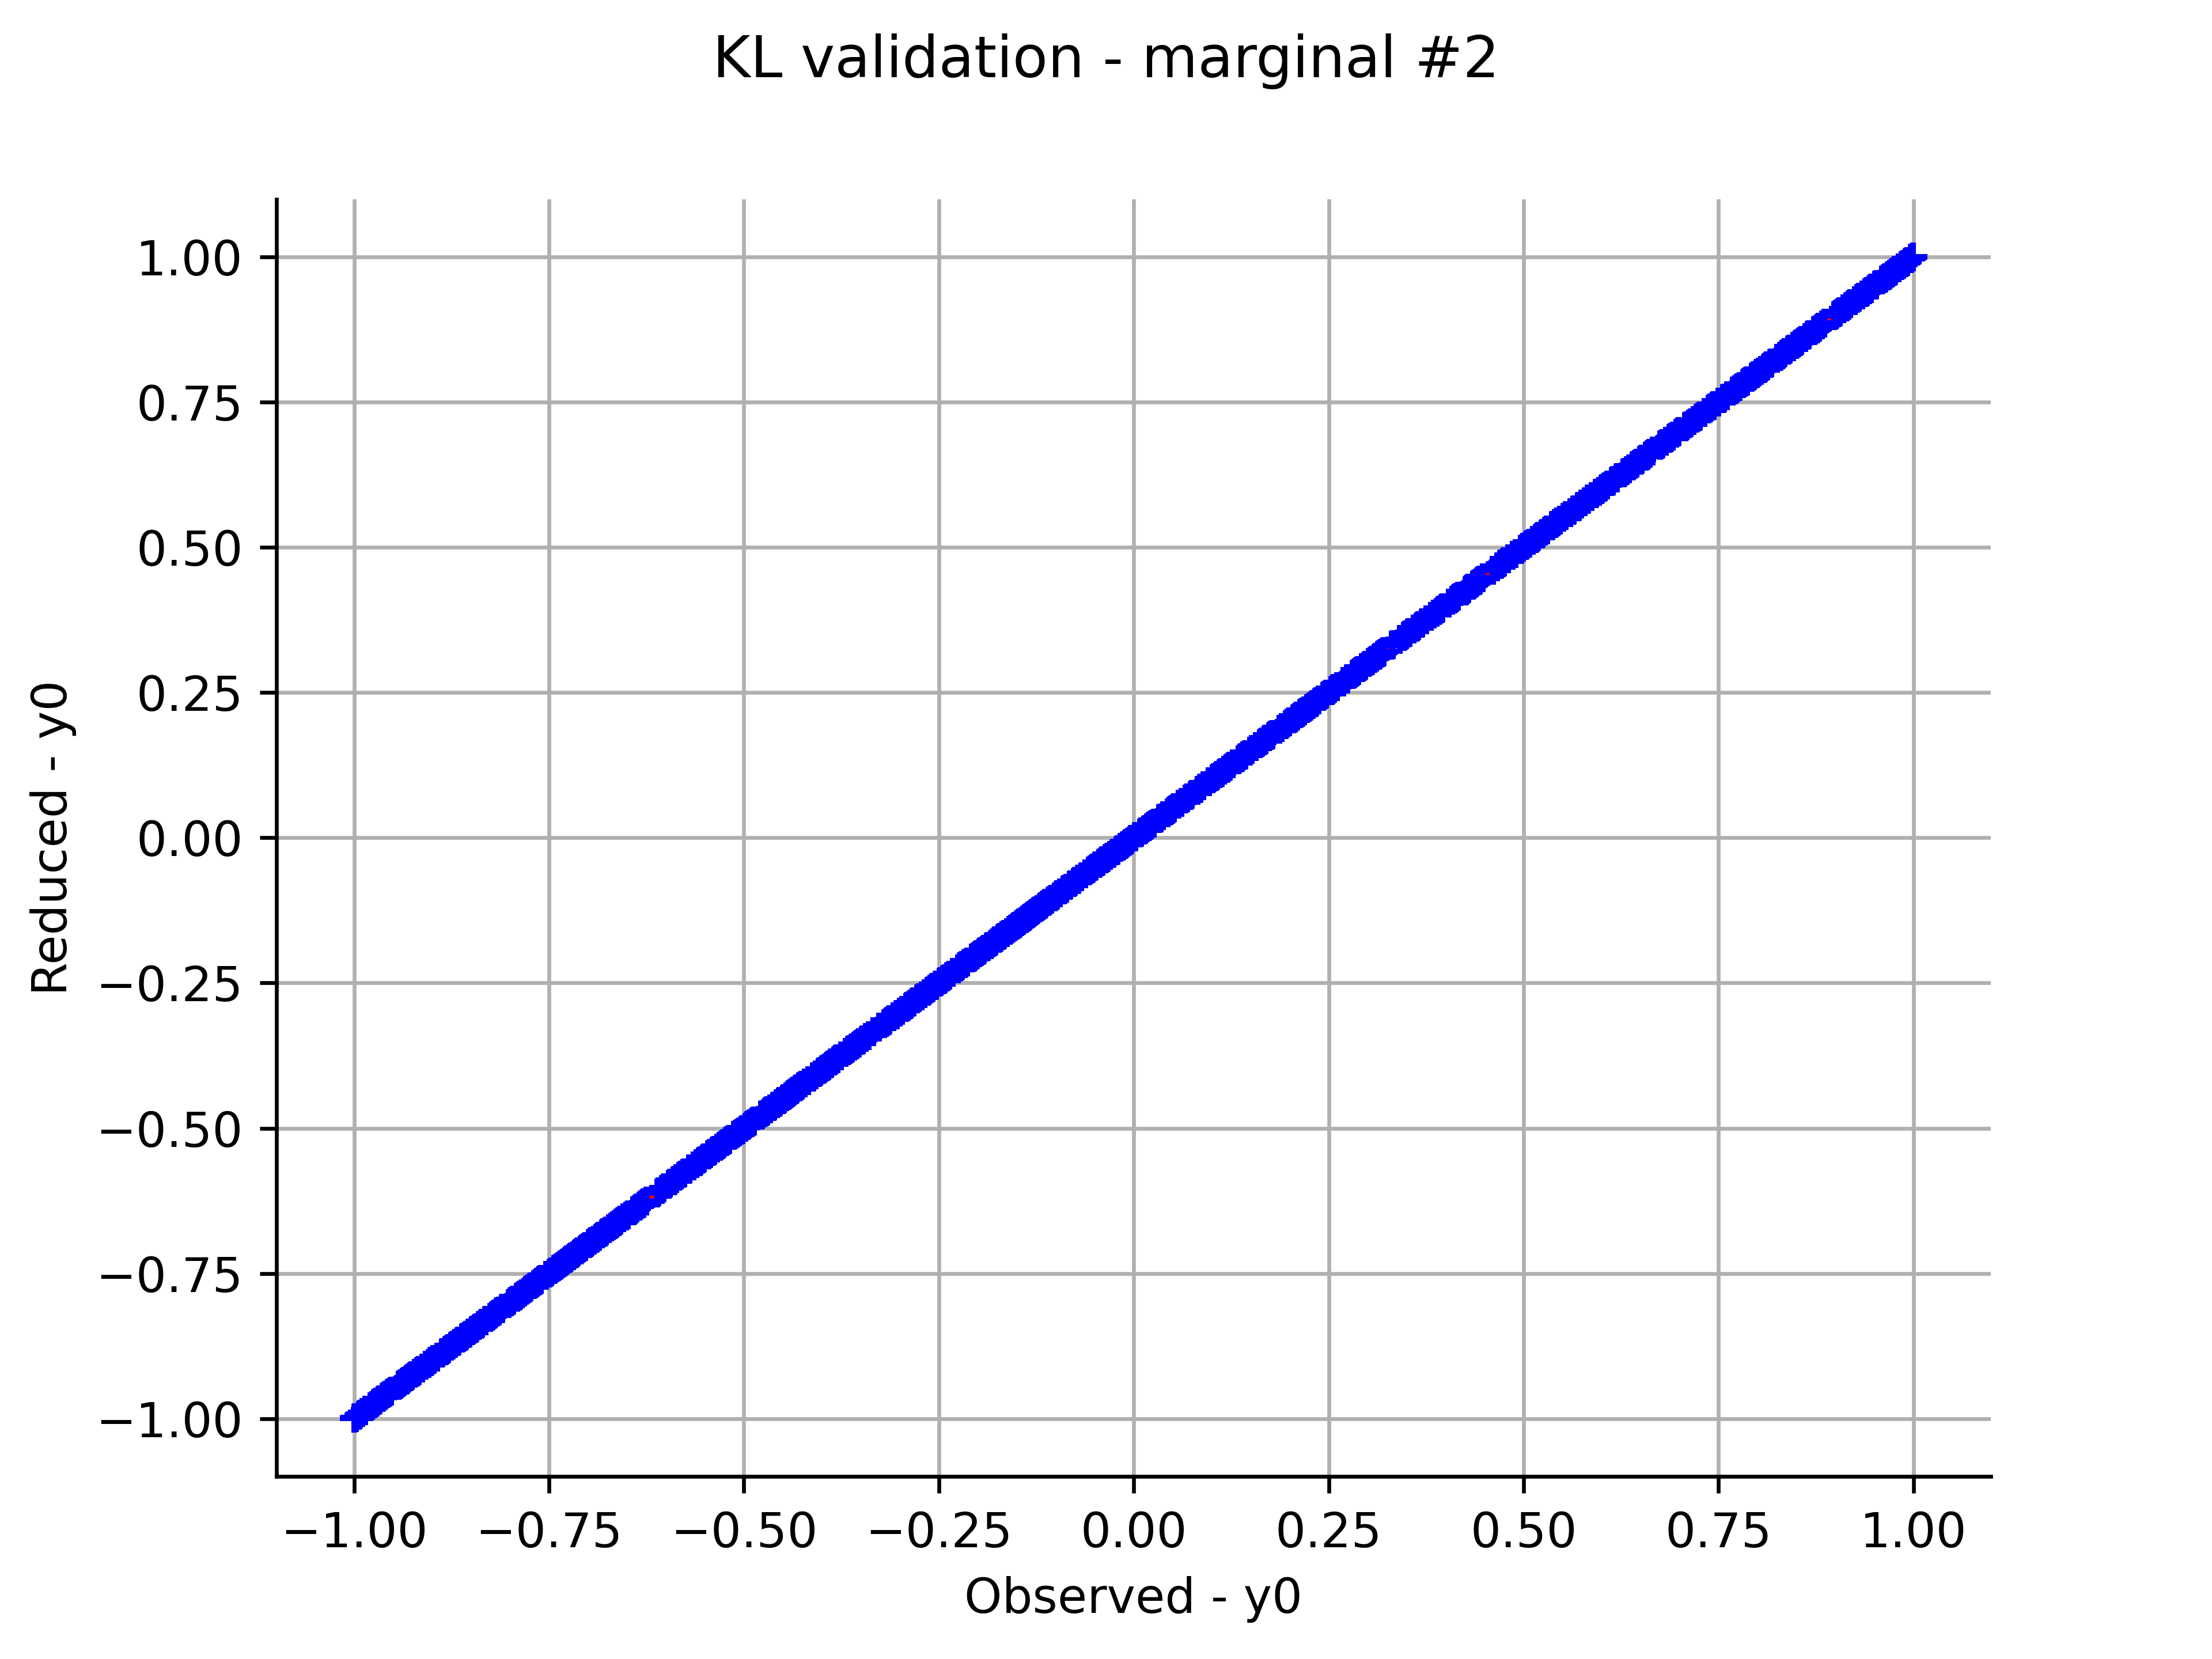
\includegraphics[width=\linewidth]{figures/valid_kl2.png}
  \caption{KL validation}
\endminipage\hfill
\minipage{0.5\textwidth}
  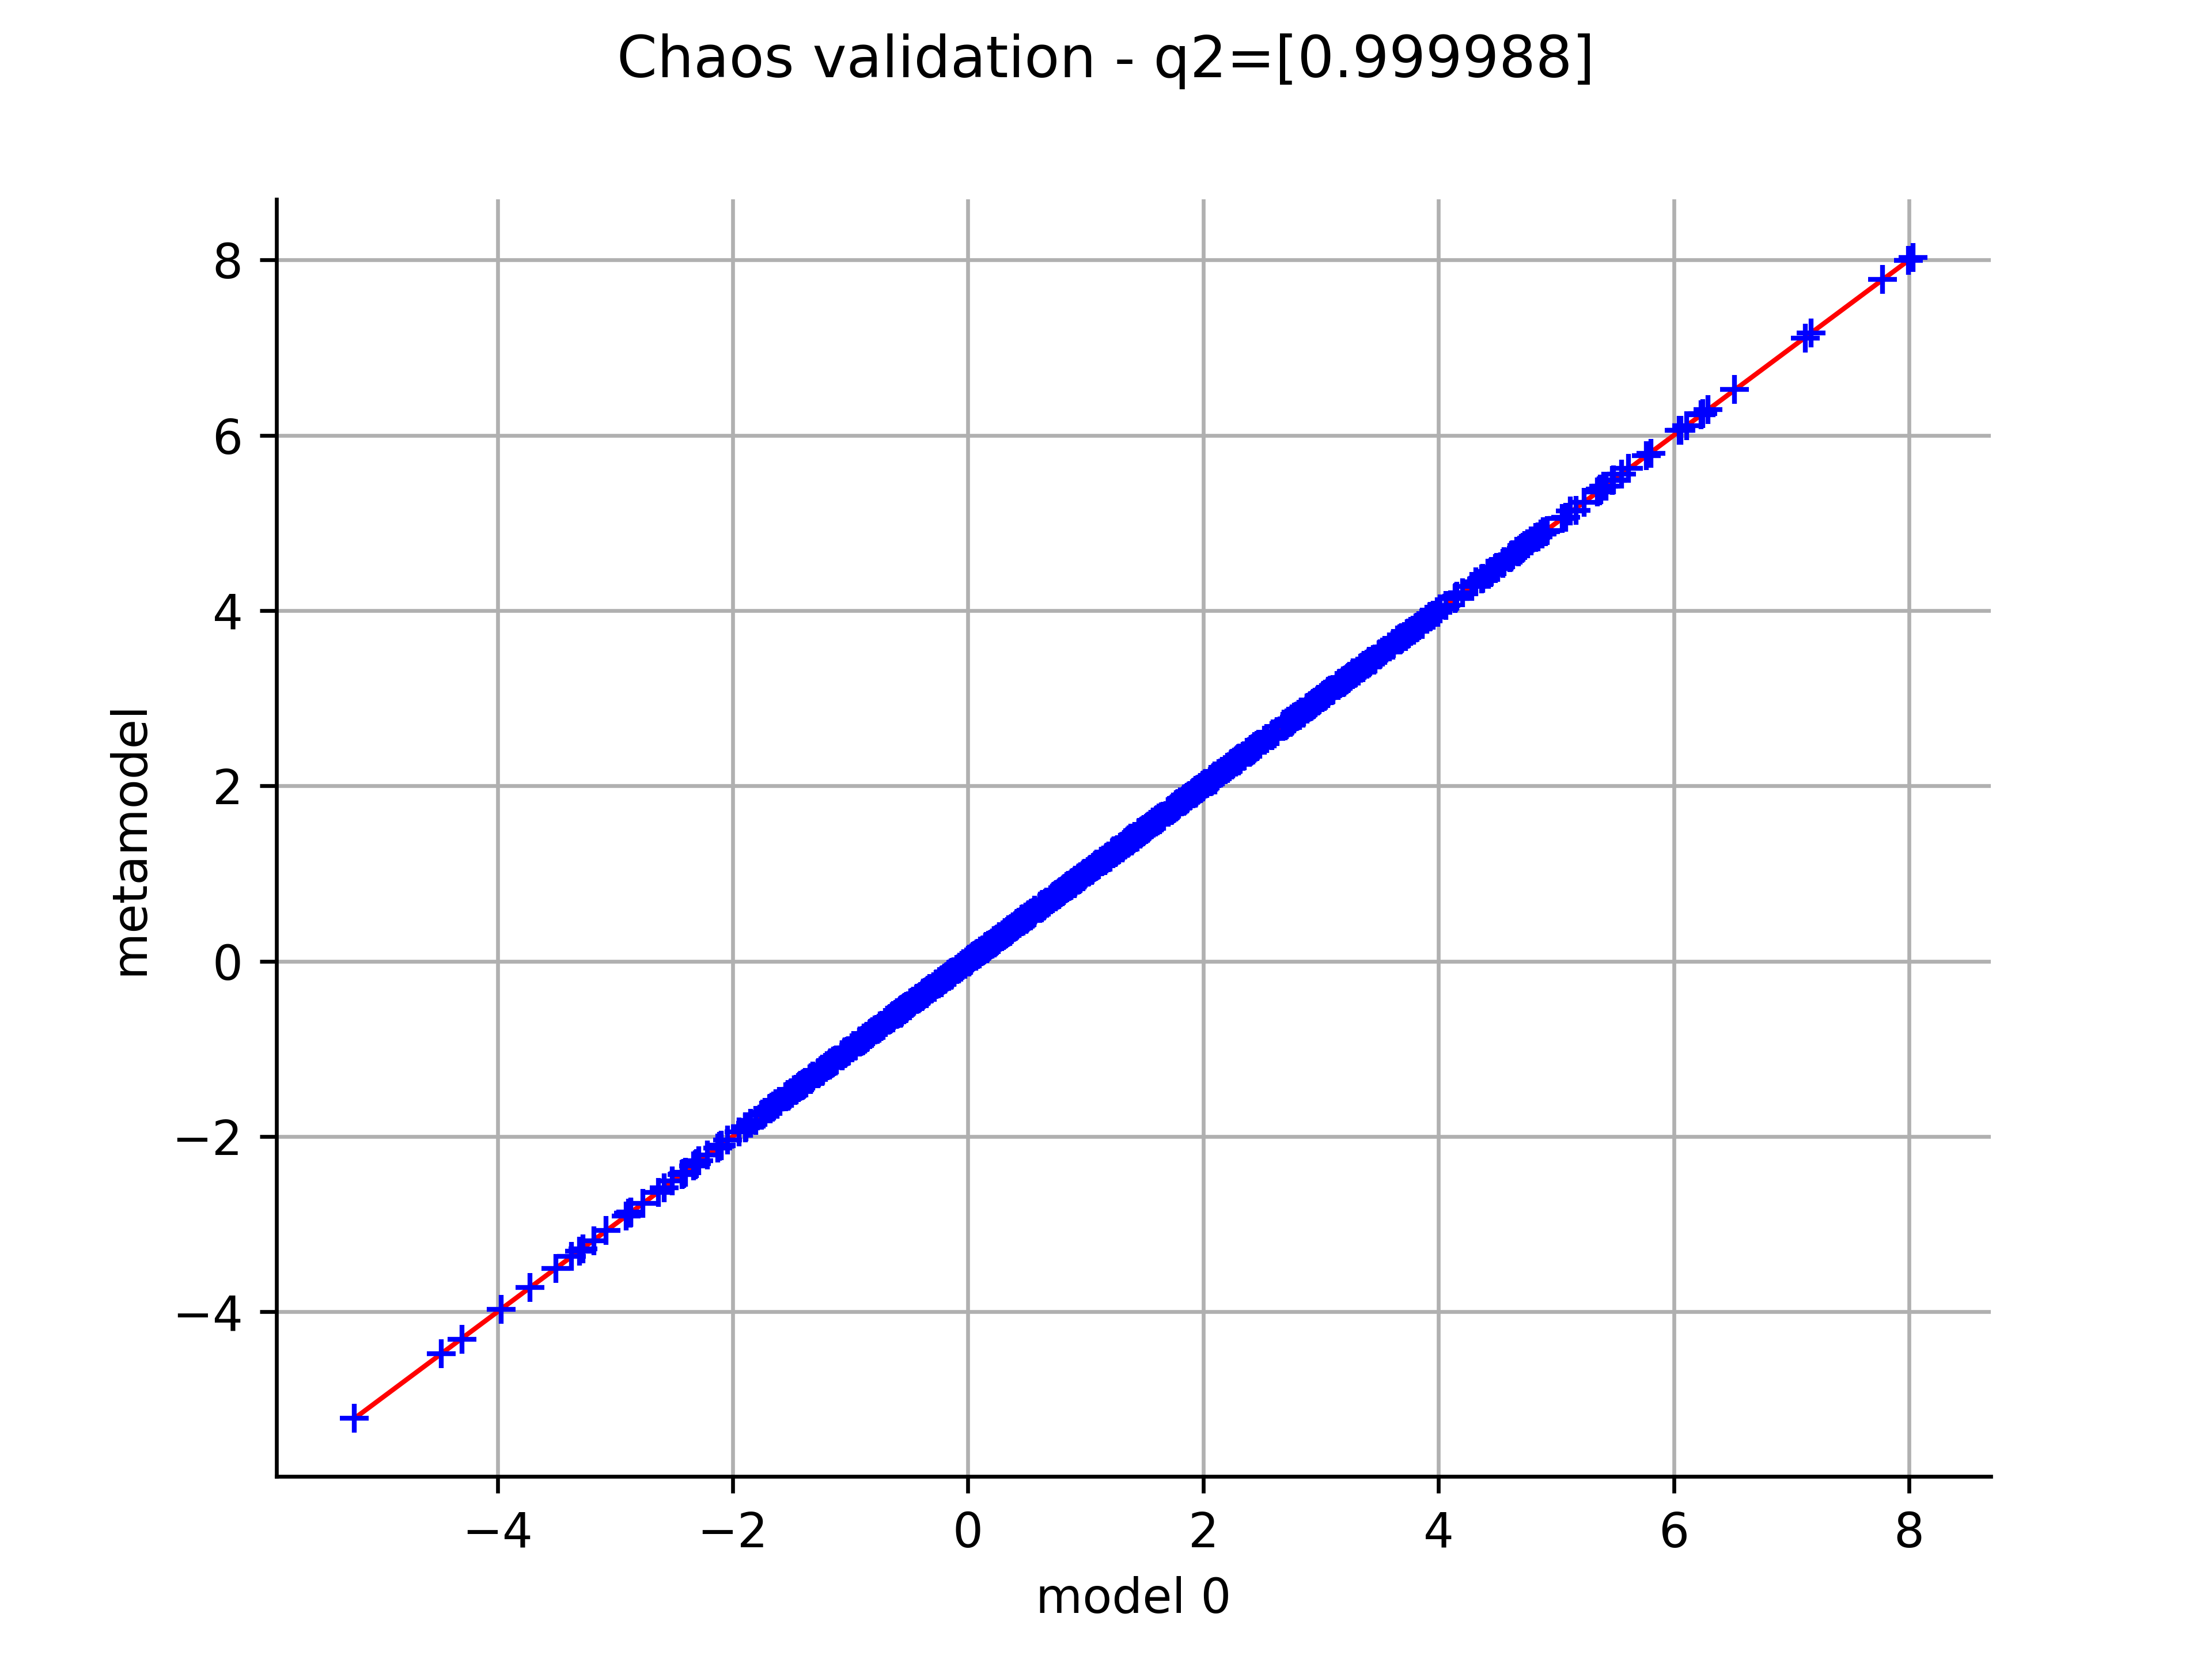
\includegraphics[width=\linewidth]{figures/valid_chaos.png}
  \caption{chaos validation}
\endminipage\hfill
\end{figure}


\end{frame}

\begin{frame}[containsverbatim]
\frametitle{Variance-based sensitivity analysis for functional inputs}

\framesubtitle{API}

\lstset{language=python}
\begin{lstlisting}

# evaluate metamodel
metamodel = result.getFieldToPointMetamodel()
y0hat = metamodel(x[0])

# retrieve Sobol indices
sobol = ot.FieldFunctionalChaosSobolIndices(result)
sobol_1 = sobol.getFirstOrderIndices()
sobol_t = sobol.getTotalOrderIndices()

# plot indices
View(sobol.draw())

# higher order indices
sobol12 = sobol.getSobolIndex([0, 1])

\end{lstlisting}

\end{frame}

\begin{frame}[containsverbatim]
\frametitle{Variance-based sensitivity analysis for functional inputs}

\framesubtitle{API}

\begin{center}
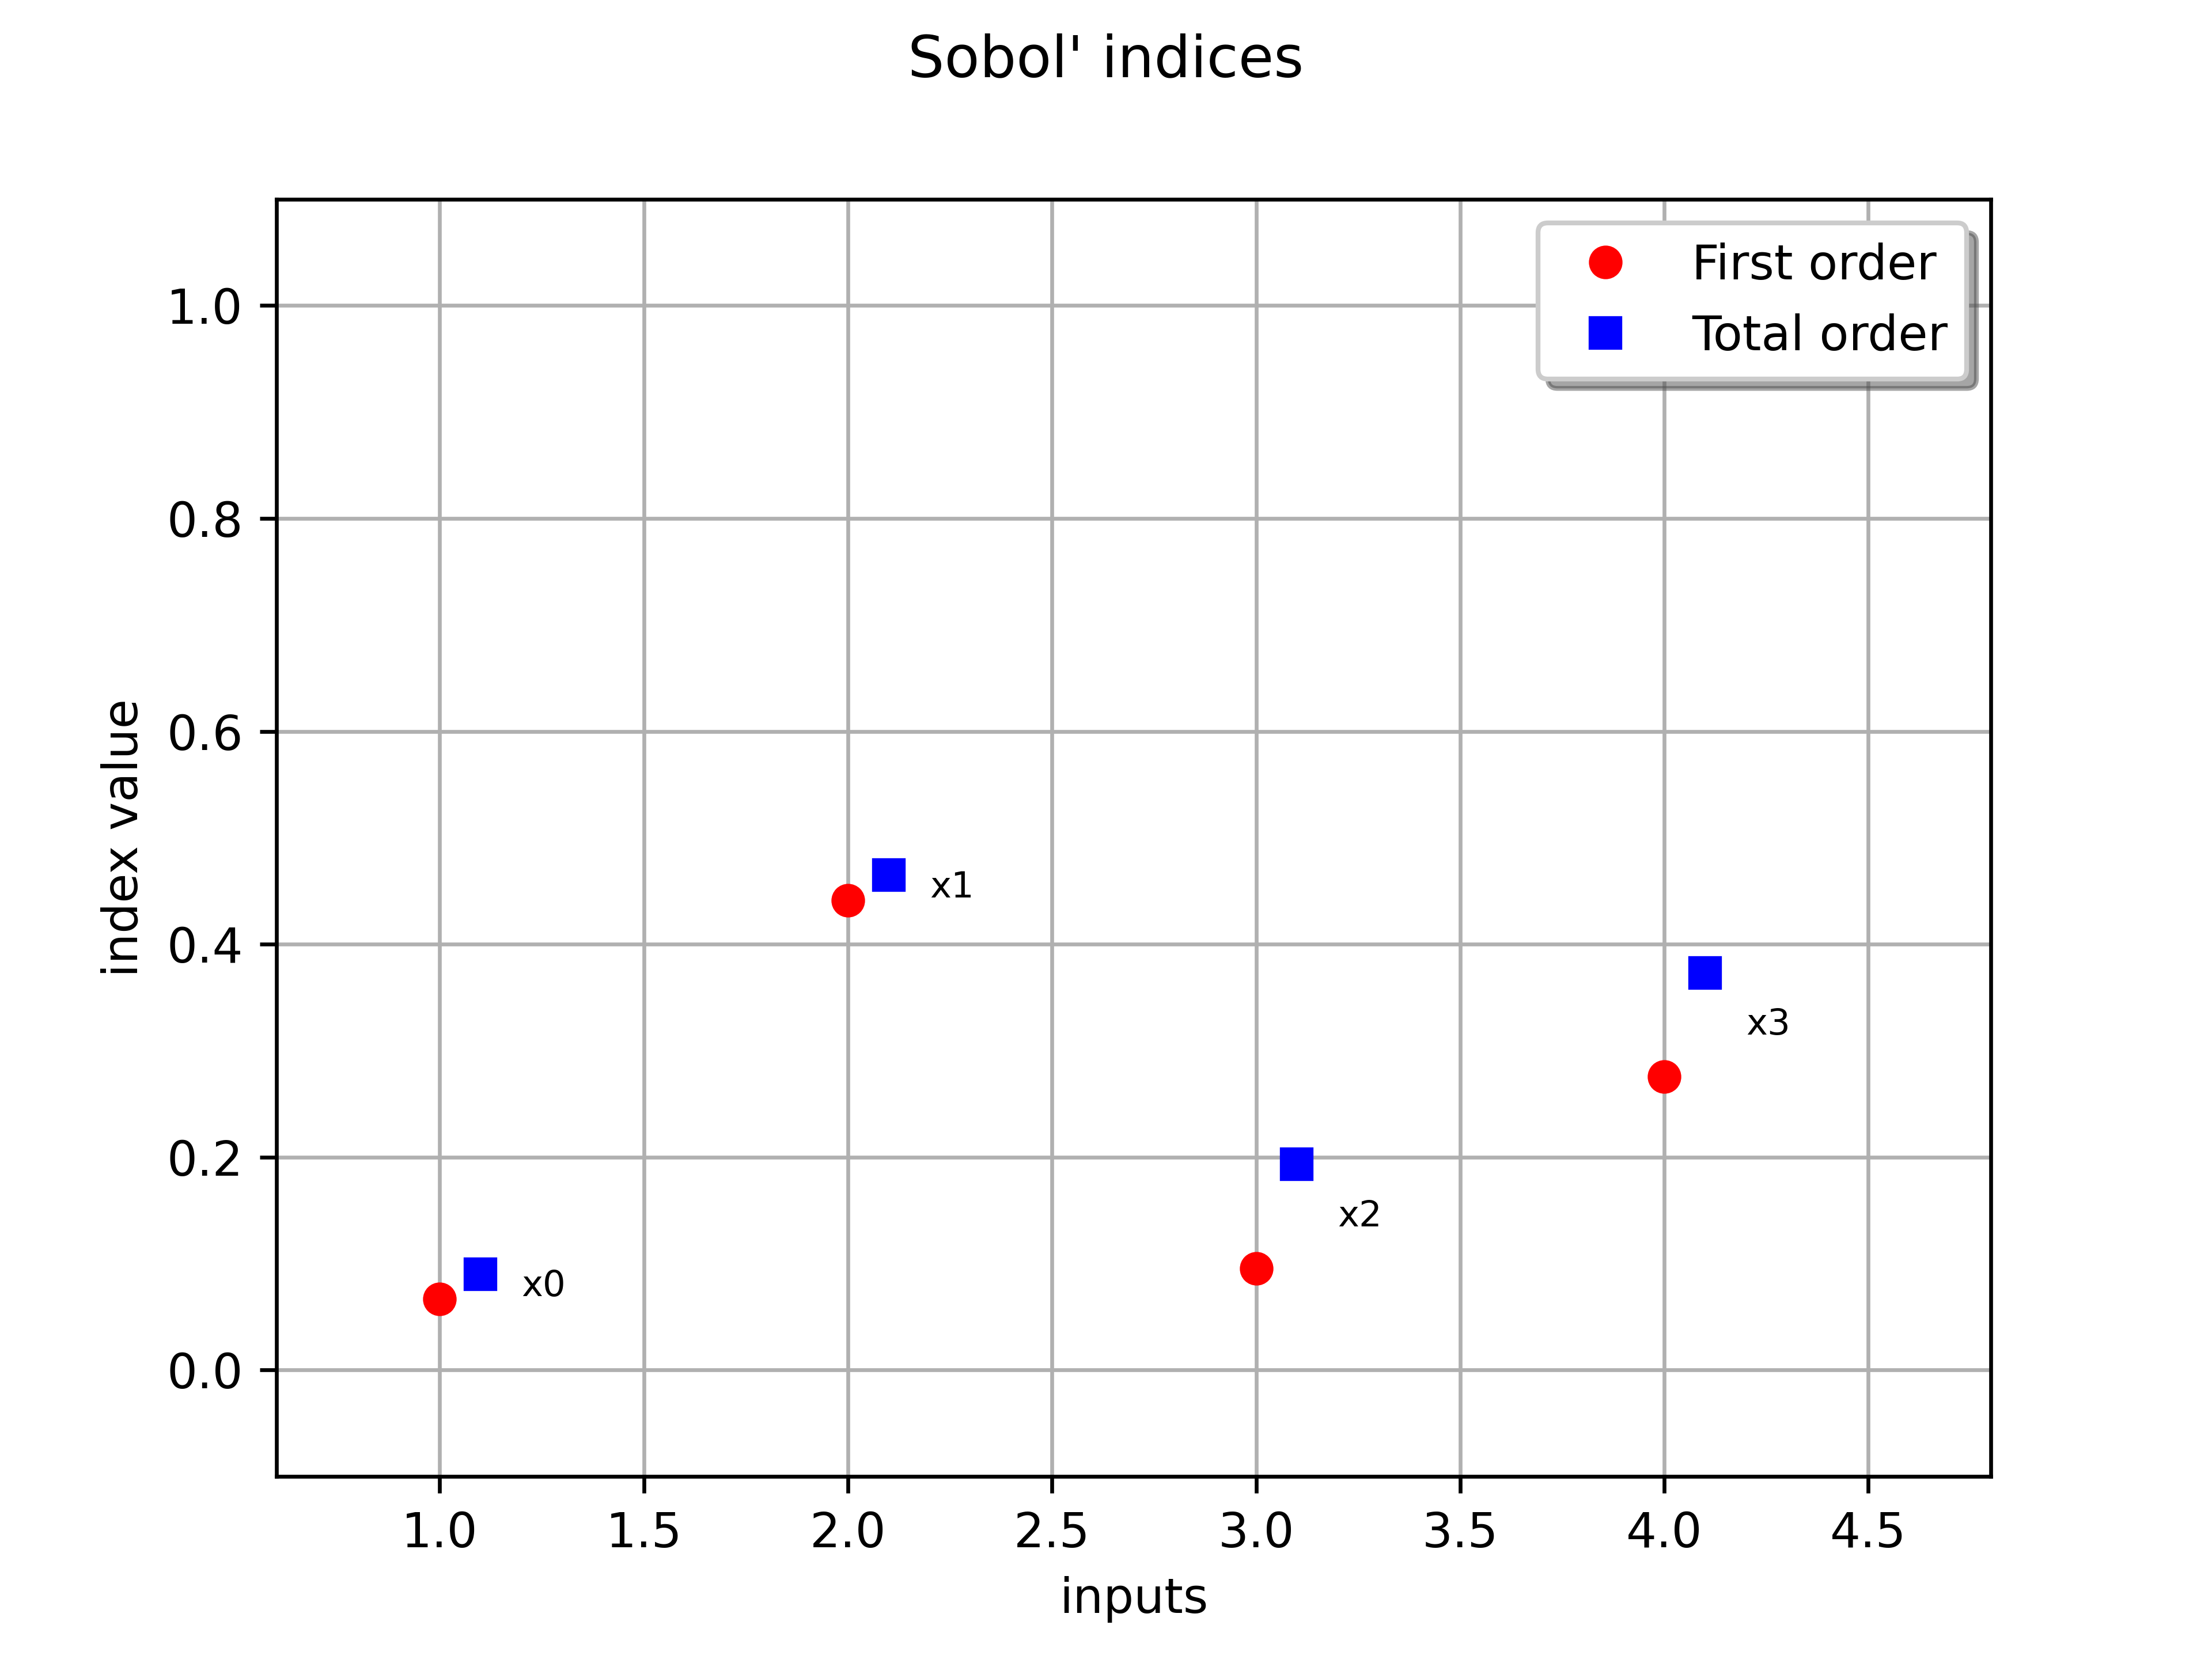
\includegraphics[width=0.6\textwidth]{figures/sobol.png}
\end{center}

\end{frame}


\begin{frame}[containsverbatim]
\frametitle{Variance-based sensitivity analysis for functional inputs}

\framesubtitle{Outlook}

\begin{itemize}
\item Development is settling down
\item Expected to land in OT 1.20 (fall 2022)
\item Extension to Vector $\mapsto$ Field, Field $\mapsto$ Field ?
\end{itemize}

\end{frame}

\end{document}
